\chapter{Implementacja programu}
W rozdziale piątym zostały przedstawione najważniejsze fragmenty sposobu implementacji programu. 

\section{Realizacja detekcji pięciolinii}
Proces digitalizacji zapisów nutowych dzisiaj odbywa się zazwyczaj przy pomocy zdjęć zrobionych przy użyciu przenośnych urządzeń, takich jak telefon wyposażony w aparat, zamiast skanerów. Jak takie podejście jest wygodniejsze dla użytkownika, gdyż w dzisiejszych czasach większość osób ma już przy sobie przez prawie cały czas urządzenia wyposażone w aparat, to niestety wszystkie układy optyczne wprowadzają dystorsję do wykonywanego obrazu, beczkową dla obiektywów szerokokątnych, czy poduszkową dla teleobiektywów, co powoduje niechciane zniekształcenia w zapisywanym obrazie. Kolejną wadą fotografowania dokumentów jest to, iż w przeciwieństwie do skanów ze skanerów, uzyskany obraz nie jest płaski i wyrównany z ewentualnym lekkim przechyleniem, które jest proste do poprawienia, tylko często posiada zniekształcenia we wszystkich wymiarach, jak na przykład gdy fotografuje się stronę książki, co skutkuje nieliniowymi wygięciami przy krawędziach stron. 

Wszelkie wprowadzone zniekształcenia mogą powodować, iż skuteczność wytrenowanego modelu do odczytywania informacji semantycznych zapisu nutowego spada, gdyż jedną z najważniejszych właściwości nuty jest jej relacja do pięciolinii, która to określa wysokość jej tonu, a wprowadzone przez fotografowanie na nierównej powierzchni nut, czy strony z książki, zniekształcenia zmniejszają skuteczność wytrenowanego modelu. Dodatkowo przy zniekształceniach wynikających z wybrzuszenia kartki, nietrywialne staje się podzielenie obrazu tak, by fragment zawierający pięciolinię przekazywany do modelu zawierał tylko interesującą nas część obrazu bez większych fragmentów pozostałej części zdjęcia, które mogą wprowadzać niechciane informacje zmniejszające skuteczność programu.



\subsection{Realizacja detekcji wypaczonych pięciolinii}
Jedną z najbardziej przydanych właściwości pięciolinii jest ich forma, mianowicie pięć prostych, równoodległych linii, co czyni je perfekcyjnymi kandydatami do detekcji zniekształceń wprowadzonych przez proces fotografowania, pozwalając na usunięcie tychże niedoskonałości geometrycznych obrazu. 

Proces detekcji pozycji wypaczonych pięciolinii na obrazie odbywa się przy pomocy analizy histogramów okienek próbnikowych. Okienkiem próbnikowym nazywany jest fragment obrazu rozciągający się na całą jego wysokość i pewną szerokość, przy pomocy którego dokonywana jest analiza obrazu, poprzez analizę mniejszych fragmentów. Po analizie jednego okienka, jego pozycja jest przesuwana o odpowiedni interwał, po czym ponownie następuje analiza danego fragmentu.

Dla ułatwienia operacji obraz zostaje konwertowany do odcieni szarości, gdyż informacje kolorystycznie nie są potrzebne do wydobywania niezbędnych z niego informacji. Następnie na obrazie dokonywane są operacje edycji, mianowicie rozmycie gaussowskie, adaptacyjne progowanie i erozja by pozostawić tylko pożądane informacje z obrazu. Kolejnym krokiem jest konwersja uzyskanego efektu do tablicy, w celu uproszczenia operacji w następnych krokach. 

Przed detekcją pozycji pięciolinii wykonywana jest operacja odnalezienia odległości między liniami pięciolinii, poprzez analizę histogramów kilku okienek próbnikowych o szerokości jednej czterdziestej obrazu. Polega to na stworzeniu histogramu występowania czarnych pikseli we wszystkich rzędach okienka, po czym następuje odfiltrowanie wartości mniejszych niż 70 procent maksymalnej wartości z histogramu, by usunąć informacje niebędące potencjalnie liniami pięciolinii, jak główki i ogonki nut oraz inne znaki zapisu nutowego. Następnie dokonuje się estymacji dokładnej pozycji linii w histogramie.

Na obrobionych w ten sposób danych dokonywane jest właściwe odszukiwanie odległości między liniami. Polega ono na zebraniu długości sekwencji pomiędzy pozycjami szczytów histogramu i odnalezieniu najczęściej występującej, regularnej z pewnym dopuszczalnym błędem, odległości.

\begin{figure}
	\centering
	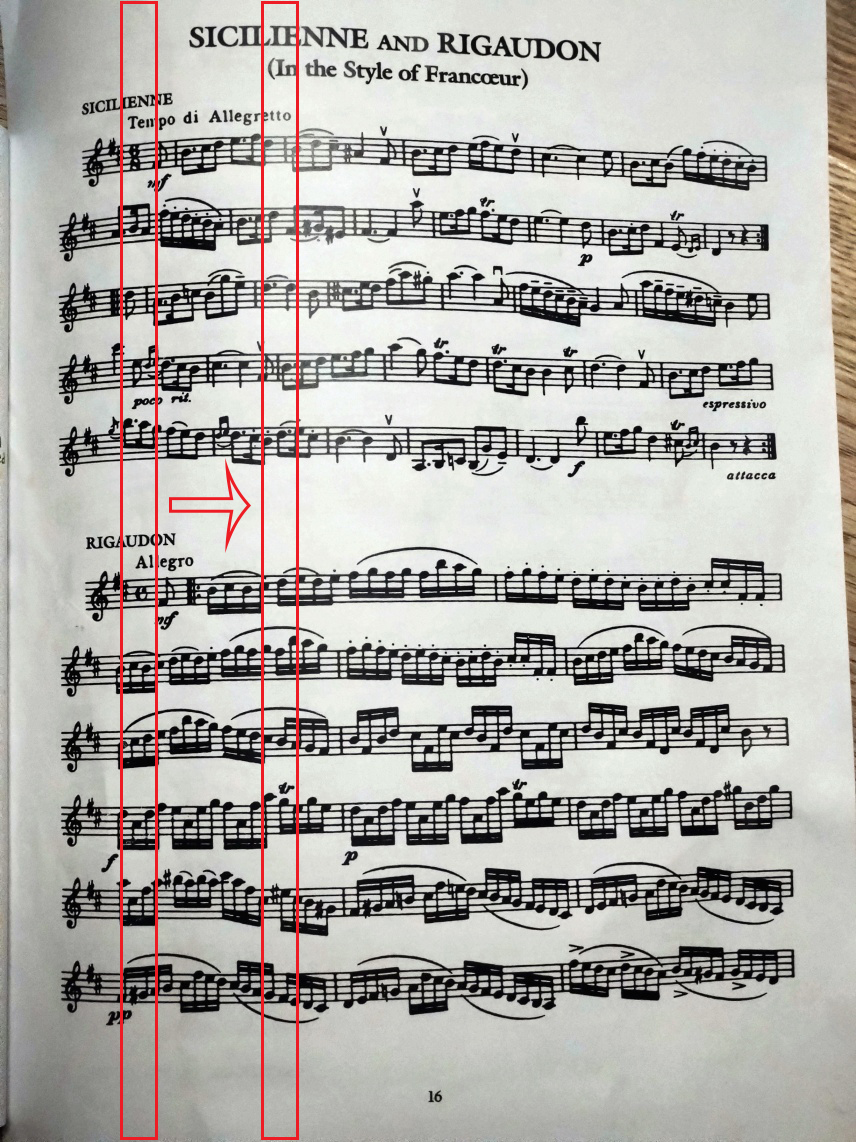
\includegraphics[width=10cm]{images/probe_window_demo.jpg}
	\caption{Wizualizacja okienka próbnikowego na zdjęciu nut.}
	\label{fig:probe_window_demo}
\end{figure}

\begin{lstlisting}
def find_staves_points(img, stride = 2):
	img = enhance_image(img)
	
	img_array = tf.keras.utils.img_to_array(img)
	img_y, img_x, c = img_array.shape
	
	staff_line_dist = find_staff_line_distance(img_x, img_y, img_array)
	if staff_line_dist == -1:
		return -1, 0
	
	staves_positions = find_staves_positions(img_x, img_y, staff_line_dist, stride, img_array)
	if len(staves_positions) == 0:
		return -1, -1
	else:
		staves_points_list = make_satves_points_list(staves_positions, staff_line_dist)
		if len(staves_points_list) == 0:
			return -1, -1
		return staves_points_list, staff_line_dist
\end{lstlisting}

\begin{lstlisting}
def find_staff_line_distance(img_x, img_y, img_array = np.array):
	probe_window_size = img_x // 40
	probe_window_start_idx = probe_window_size * 5
	probe_window_hist_arr = np.zeros(img_y)
	staff_line_distance_list = []
	
	for i in range(probe_window_start_idx, img_x, probe_window_size * 5):
		if i > img_x - probe_window_size * 2:
			break
		
		for j in range(i, i + probe_window_size):
			for k in range(0, img_y):
				if img_array[k][j] < 200:
					probe_window_hist_arr[k] += 1
	
	peaks_list = filter_out_stave_lines(probe_window_size, probe_window_hist_arr)
	
	staff_line_distance = find_staff_line_distance_in_probe(peaks_list)
	if staff_line_distance != 0:
		staff_line_distance_list.append(staff_line_distance)
	
	if len(staff_line_distance_list) != 0:
		return sum(staff_line_distance_list) // len(staff_line_distance_list)
	else:
		return -1
\end{lstlisting}


\begin{lstlisting}
def find_staves_positions(img_x, img_y, staff_line_distance, stride = 1, img_array = np.array):
	probe_window_size = staff_line_distance * 2 + 5
	probe_window_start_idx = probe_window_size * 2
	probe_window_hist_arr = np.zeros(img_y)
	staves_positions_list = []
	for i in range(probe_window_start_idx, img_x, probe_window_size * stride):
		if i > img_x - probe_window_size * 2:
			break
	
		for j in range(i, i + probe_window_size):
			for k in range(0, img_y):
				if img_array[k][j] < 200:
					probe_window_hist_arr[k] += 1
		
		peaks_list = filter_out_stave_lines(probe_window_size, probe_window_hist_arr)
		
		staves_positions = get_staves_positions(i, staff_line_distance, peaks_list)
		staves_positions_list.append(staves_positions)
		
		probe_window_hist_arr = np.zeros(img_y)
	
	if len(staves_positions_list) == 0:
		return -1
	else:
		return staves_positions_list
\end{lstlisting}


\section{Usuwanie wypaczania obrazu}

\section{Segmentacja obrazu}

\section{Model głębokiego uczenia do rozpoznawania zapisu nutowego}

